%!TEX root = /Users/andrea/Unive/Specialistica/Artificial Intelligence/Mod. A/dispensa/main.tex

\chapter{Modello Neurale} % (fold)
\label{cha:modello_neurale}
Le reti neurali artificiali sono nate per riprodurre attività tipiche del cervello umano come la percezione di immagini, il riconoscimento di forme, la comprensione del linguaggio, il coordinamento senso-motorio, ecc. A tale scopo si sono studiate le caratteristiche del cervello umano.\\									

Nel sistema nervoso esistono miliardi di neuroni (cellule nervose).
Nel modello biologico un \textbf{neurone} è caratterizzato da:
\begin{itemize}
    \item \textbf{corpo cellulare (soma)}: l'unità di calcolo del neurone (5/10 micron);
    \item \textbf{assone}: meccanismo di output di un neurone;
    \item \textbf{dendriti}: ricevono segnali in input da altri assoni tramite le \textbf{sinapsi}
\end{itemize}

\begin{figure}[h!]
    \centering
    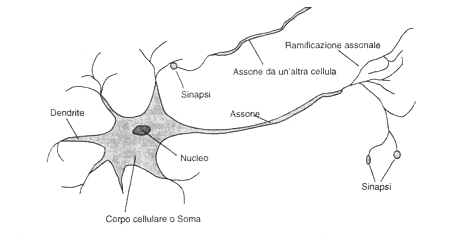
\includegraphics[width=\textwidth]{images/neuron.png}
    \caption{Neuroni biologici}\label{fig:neuron}
\end{figure}

All’estremità l'assone si ramifica formando terminali attraverso i quali i segnali elettrici vengono trasmessi ad altre cellule (ad esempio ai dendriti di altri neuroni). Tra un terminale di un assone e la cellula ricevente esiste uno spazio. I segnali superano questo spazio per mezzo di sostanze chimiche dette \emph{neurotrasmettitori}. Il punto di connessione tra terminale e dendrite è detto \textbf{sinapsi}.

\newpage
La trasmissione di un segnale nella corteccia cerebrale è un processo complesso.
In maniera molto semplificata, tale processo si compone delle seguenti fasi:
\begin{enumerate}
    \item Il corpo cellulare esegue una somma pesata dei segnali in ingresso;
    \item Se il risultato supera un certo valore soglia allora si produce un \textbf{potenziale d'azione}; una scarica di impulsi elettrici, che viene inviata all'assone. In questo caso, si dice che la cellula ``spari'' altrimenti non fa nulla;
    \item Quando il segnale elettrico raggiunge la sinapsi, viene rilasciato chimicamente un “neuro trasmettitore” che sarà combinato con i “recettori” nella membrana post-sinaptica (vedi Figura~\ref{fig:synapse});
    \item I recettori post-sinaptici provocano una diffusione del segnale elettrico nel neurone post-sinaptico.
\end{enumerate}

\begin{figure}[h!]
    \centering
    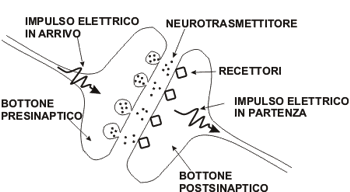
\includegraphics[width=8cm]{images/synapse.png}
    \caption{La sinapsi}\label{fig:synapse}
\end{figure}
\emph{L'apprendimento} si attua modificando la cosiddetta \textbf{efficacia sinaptica}, ovvero l'ammontare di corrente che entra nel neurone post-sinaptico rispetto al potenziale d'azione del neurone pre-sinaptico. In questo contesto le sinapsi possono essere: \textbf{eccitatorie}, nel senso che favoriscono la generazione di potenziale d'azione nel neurone post-sinaptico, oppure \textbf{inibitorie} che, invece, ne limitano la generazione.
Il cervello umano è un calcolatore complesso, non lineare e parallelo. Pur essendo costituito da elementi di elaborazione molto semplici (i neuroni), è in grado di eseguire computazioni complesse, come il riconoscimento, la percezione e il controllo del movimento, molte volte più velocemente del più veloce degli attuali calcolatori.\\

Nel cervello non esiste un controllo centralizzato, nel senso che le varie zone del cervello funzionano insieme, influenzandosi reciprocamente e contribuendo alla realizzazione di uno specifico compito.

\newpage

Infine, il cervello è \emph{fault tolerant}, cioè se un neurone o una delle sue connessioni sono danneggiati, il cervello continua a funzionare, anche se con prestazioni leggermente degradate. In particolare, le prestazioni del processo cerebrale degradano gradualmente man mano che si distruggono sempre più neuroni (\emph{graceful degradation}).
A tale scopo si sono studiate le caratteristiche del cervello umano.
Quindi, per riprodurre artificialmente il cervello umano occorre realizzare una rete di elementi molto semplici che sia una struttura \textbf{distribuita}, massicciamente \textbf{parallela}, capace di \textbf{apprendere} e quindi di \textbf{generalizzare} (cioè produrre uscite in corrispondenza di ingressi non incontrati durante l’addestramento).\\

Il metodo più usato per addestrare una rete neurale consiste nel presentare in ingresso alla rete un insieme di esempi (training set). La risposta fornita dalla rete per ogni esempio viene confrontata con la risposta desiderata, si valuta la differenza (errore) fra le due e, in base a tale differenza, si aggiustano i pesi. Questo processo viene ripetuto sull’intero training set finché le uscite della rete producono un errore al di sotto di una soglia prestabilita.\\

Anche se di recente introduzione, le reti neurali trovano valida applicazione in settori quali predizione, classificazione, riconoscimento e controllo, portando spesso contributi significativi alla soluzione di problemi difficilmente trattabili con metodologie classiche.

\newpage

\section{Modello di McCulloch e Pitts} % (fold)
\label{sec:modello_di_mcculloch_e_pitts}
Si introduce ora un modello artificiale del neurone biologico. Il neurone artificiale ha molti ingressi ed una sola uscita. Ogni ingresso ha associato un peso, che determina la conducibilità del canale di ingresso. L’attivazione del neurone è una funzione della somma pesata degli ingressi.

\begin{figure}[h!]
    \centering
    \begin{tikzpicture}[shorten >=1pt, node distance=\layersep]
        % Draw the input layer nodes
        \foreach \name / \y in {1,...,4}
        % This is the same as writing \foreach \name / \y in {1/1,2/2,3/3,4/4}
            \node[input neuron, pin=left:$n_\y$] (I-\name) at (0,-\y) {};
        \node[input neuron,  pin=left:$n_n$] (I-5) at (0,-6) {};
        \draw[dotted, thick] (I-4) -- (I-5);
        % Draw the output layer node
        \node[output neuron, right of=I-3] (O) {$\Sigma$};
        \node[neuron, right of=O, pin={[pin edge={<-}]above:$\mu_i$}] (F) {$\Theta(x)$};
        \node[right of=F] (Y) {Output};
        \path (O) edge [->] (F)
         (F) edge [->] (Y);
        % Connect every node in the hidden layer with the output layer
        \foreach \source in {1,...,4}
            \path (I-\source) edge [->, above] node {\scriptsize$w_{i\source}$} (O);
        \path (I-5) edge [->] node [above=0.3cm of I-5] {\scriptsize$w_{in}$} (O);
        \node[above=0.5cm of I-1] {Input layer};
        \node[above=2.5cm of F] {Output layer};
    \end{tikzpicture}
    \caption{Neurone artificiale nel modello M\&P}
\end{figure}

Un insieme di neuroni artificiali forma una \emph{rete artificiale}. Una rete neurale è un grafo diretto pesato aciclico $N=(V,E,w)$ dove $V=\{ 0,1,\dots, n\}$ è l'insieme delle unità (o neuroni), $E \subseteq V \times V$ è l'insieme di connessioni e $w:E \rightarrow \mathbb{R}$ è una funzione che assegna un peso con valore reale $w(i,j)$ per ogni connessione $(i,j)\in E$.\\

I pesi rappresentano l'efficacia sinaptica: pesi positivi amplificano il segnale, mentre quelli negativi lo inibiscono. Come notazione sarà utilizzata $w_{ij}$ anziché $w(i,j)$.\\

Un neurone si attiva se la somma pesata $\sum_j w_{ij} n_j$ degli input supera un certo valore soglia $\mu_i$. In termini matematici:
\begin{align}
    n_i(t + 1) = \Theta\left(\sum_j w_{ij} n_j(t) - \mu_i \right)
\end{align}

\newpage

Si tratta di un \textbf{modello semplificato} dove $\Theta(x)$ è la funzione di transizione o di attivazione ed in questo caso è lineare.
\begin{align}
    n_i(t + 1) =
    \begin{cases}
        1 & \mbox{if } \displaystyle\sum_j w_{ij} n_j \geq \mu_i \\
        0 & \mbox{otherwise} 
    \end{cases}
\end{align}

Anziché utilizzare una funzione discreta si possono adottare funzioni continue in modo tale da rendere il sistema più realistico. In questa caso l'output corrisponde alla frequenza delle volte in cui un neurone tramette. Esistono diverse funzioni di transizione continue; le più usate sono la sigmoidea e la tangente iperbolica.\\

\begin{figure}[h!]
	\begin{center}
	\subfigure[Tangente iperbolica]{
    \begin{tikzpicture}[domain=-1:1,scale=1.5]
        \draw[->] (-1,0) -- (1,0) node[right] {\tiny$x$};
        \draw[->] (0,-1.2) -- (0,1.2) node[above] {\tiny$f(x)$};
		\draw[dashed, thin] plot function{1} node[above]{\tiny +1};
		\draw[dashed, thin] plot function{-1} node[above]{\tiny-1};
        \draw[color=blue, thick] plot[id=tanh] function{tanh(x)};
    \end{tikzpicture}}
	\qquad
	\subfigure[Lineare]{
    \begin{tikzpicture}[domain=-1:1,scale=1.5]
        \draw[->] (-1,0) -- (1,0) node[right] {\tiny$x$};
        \draw[->] (0,-1.2) -- (0,1.2) node[above] {\tiny$f(x)$};
		\draw[dashed, thin] plot function{1} node[above]{\tiny +1};
		\draw[dashed, thin] plot function{-1} node[above]{\tiny-1};
        \draw[color=red, thick] plot[id=x] function{x};
    \end{tikzpicture}}
	\qquad
	\subfigure[Sigmoidea]{
    \begin{tikzpicture}[domain=-1:1,scale=1.5]
        \draw[->] (-1,0) -- (1,0) node[right] {\tiny$x$};
        \draw[->] (0,-1.2) -- (0,1.2) node[above] {\tiny$f(x)$};
		\draw[dashed, thin] plot function{1} node[above]{\tiny +1};
        \draw[color=orange, thick] plot[id=sigmoidal] function{1 / (1 +  exp(- 10 * x))};
    \end{tikzpicture}}
	\caption{Le funzioni di attivazione più utilizzate.}
	\end{center}
\end{figure}

Lo scopo delle funzioni di attivazione è ridurre la varianza in output di un neurone mappando il risultato della somma pesata entro un intervallo; generalmente compreso tra $[-1, 1]$ oppure $[0, 1]$.

\newpage

\subsection{Proprietà del modello M\&P} % (fold)
\label{sub:proprietà_del_modello}
Combinando opportunamente i neuroni di M\&P si possono costruire reti in grado di realizzare qualsiasi operazione del calcolo proposizionale.

\begin{figure}[h!]
    \centering

    \subfigure[AND]{
    \begin{tikzpicture}[node distance=\layersep]]
        \node[input neuron] (I-1) at (0,1) {1};
        \node[input neuron] (I-2) at (0,3) {0};
        \node[output neuron, pin={[pin edge={<-}]above:$\mu=\frac{3}{2}$}, right of=I] (S) at (0,2) {1};
        \node[right of=S] (O) {0};
        \path 
        (I-1) edge[->] node[above] {1} (S)
        (I-2) edge[->] node[above] {1} (S)
        (S) edge[->] node[above] {$1 \leq \frac{3}{2}$} (O);
    \end{tikzpicture}}
    \qquad
    \subfigure[OR]{
    \begin{tikzpicture}[node distance=\layersep]]
        \node[input neuron] (I-1) at (0,1) {1};
        \node[input neuron] (I-2) at (0,3) {0};
        \node[output neuron, pin={[pin edge={<-}]above:$\mu=\frac{1}{2}$}, right of=I] (S) at (0,2) {1};
        \node[right of=S] (O) {1};
        \path 
        (I-1) edge[->] node[above] {1} (S)
        (I-2) edge[->] node[above] {1} (S)
        (S) edge[->] node[above] {$1 \geq \frac{1}{2}$} (O);
    \end{tikzpicture}}
    \subfigure[NOT]{
    \begin{tikzpicture}[node distance=\layersep]]
        
        \node[input neuron] (I) {1};
        \node[output neuron, pin={[pin edge={<-}]above:$\mu=\frac{1}{2}$}, right of=I] (S) {-1};
        \node[right of=S] (O) {0};
        \path 
        (I) edge[->] node[above] {-1} (S)
        (S) edge[->] node[above] {$-1 \leq \frac{1}{2}$} (O);
    \end{tikzpicture}}
    \caption{Operazioni logiche elementari nel modello M\&P.}
\end{figure}

È importante notare che in questo modello \textbf{non} avviene ancora nessun tipo apprendimento. I pesi, infatti, rimangono fissi; l'apprendimento si realizza attraverso la variazione/aggiornamento dei pesi sinaptici.
% subsection proprietà_del_modello (end)
% section modello_di_mcculloch_e_pitts (end)

\newpage

\section{Tipi di architetture della rete} % (fold)
\label{sec:tipi_di_architetture_della_rete}
Il modo con cui è strutturata la rete dipende dall'algoritmo di apprendimento che si ha intenzione di usare. In generale si identificano tre classi di reti:
\begin{itemize}
    \item \textbf{reti feedforward ad uno strato}: In questa forma semplice di rete a strati, abbiamo i nodi di input (input layer) e uno strato di neuroni (output layer). Il segnale nella rete si propaga in avanti in modo aciclico, partendo dal layer di input e terminando in quello di output;
    \begin{figure}[h!]
        \centering
        \begin{tikzpicture}[->, node distance=\layersep]

            % Draw the input layer nodes
            \foreach \name / \y in {1,...,3}
                \node[input neuron] (I-\name) at (0,-\y) {};

            % Draw the output layer nodes
            \foreach \name / \y in {1,...,2}   
                \node[output neuron] (O-\name) at (\layersep, -\y cm - 0.5cm) {};

            % Connect every node in the input layer with every node in the output layer.
            \foreach \source in {1,...,3}
                \foreach \dest in {1,...,2}
                    \path (I-\source) edge (O-\dest);
                    
            % Annotate the layers
            \node[annot,above of=I-1, node distance=1cm] (il) {Input layer};
            \node[annot,right of=il] {Output layer};
        \end{tikzpicture}
        \caption{Rete forward ad uno strato}
    \end{figure}
    
    \item \textbf{reti feedforward a più strati:} questa classe di reti feedforward si distingue dalla precedente dal fatto che tra lo strato di input e quello di output abbiamo uno o più strati di neuroni nascosti (\textbf{hidden layers}).
Questo tipo di architettura fornisce alla rete una prospettiva globale in quanto aumentano le interazioni tra neuroni;
    \begin{figure}[h!]
        \centering
        \begin{tikzpicture}[->, node distance=\layersep]

            % Draw the input layer nodes
            \foreach \name / \y in {1,...,4}
                \node[input neuron] (I-\name) at (0,-\y) {};

            % Draw the hidden layer nodes
            \foreach \name / \y in {1,...,3}
            \path[yshift=2cm]
                node[hidden neuron] (H-\name) at (\layersep, -\y cm - 2.5 cm) {};

            % Draw the output layer nodes
            \foreach \name / \y in {1,...,2}   
                \node[output neuron] (O-\name) at (2*\layersep, -\y cm - 1cm) {};

            % Connect every node in the input layer with every node in the hidden layer.
            \foreach \source in {1,...,4}
                \foreach \dest in {1,...,3}
                    \path (I-\source) edge (H-\dest);
                    
            % Connect every node in the hidden layer with every node in the ouput layer.
            \foreach \source in {1,...,3}
                \foreach \dest in {1,...,2}
                    \path (H-\source) edge (O-\dest);
                    
            % Annotate the layers
            \node[annot,above of=H-1, node distance=1.5cm] (hl) {Hidden layer};
            \node[annot,left of=hl] {Input layer};
            \node[annot,right of=hl] {Output layer};
        \end{tikzpicture}
        \caption{Rete forward a più strati}
    \end{figure}
    
    \newpage
    
    \item \textbf{reti feedback o ricorrenti}: una rete ricorrente si distingue dalle precedenti nel fatto che è ciclica. La presenza di cicli ha un impatto profondo sulle capacità di apprendimento della rete e sulle sue performance, in particolare rendono il sistema \textbf{dinamico}.
    
    \begin{figure}[h!]
        \centering
        \begin{tikzpicture}[->, node distance=\layersep]

            % Draw the input layer nodes
            \foreach \name / \y in {1,...,3}
                \node[input neuron] (I-\name) at (0,-\y) {};

            % Draw the output layer nodes
            \foreach \name / \y in {1,...,2}   
                \node[output neuron] (O-\name) at (\layersep, -\y cm - 0.5cm) {};

            % Connect every node in the input layer with every node in the output layer.
            \foreach \source in {1,...,3}
                \foreach \dest in {1,...,2}
                    \path (I-\source) edge (O-\dest);
                    
            % Connect every node in the output layer with every node in the ouptu layer.
            \foreach \source in {1,...,2}
                \foreach \dest in {1,...,2} 
                {
                    \ifnum \source < \dest
                        \path (O-\source) edge [bend left] (O-\dest);
                    \fi
                    \ifnum \source > \dest
                        \path (O-\source) edge [bend left] (O-\dest);
                    \fi
                }
            % Annotate the layers
            \node[annot,above of=I-1, node distance=1cm] (il) {Input layer};
            \node[annot,right of=il] {Output layer};
        \end{tikzpicture}
        \caption{Rete  feedback.}
    \end{figure}
    
\end{itemize}
% section tipi_di_architetture_della_rete (end)
% chapter reti_neurali (end)
